%% 2-column papers and discussion papers
\documentclass[gmd, manuscript]{copernicus}

%% \usepackage commands included in the copernicus.cls:
%\usepackage[german, english]{babel}
%\usepackage{tabularx}
%\usepackage{cancel}
%\usepackage{multirow}
%\usepackage{supertabular}
%\usepackage{algorithmic}
%\usepackage{algorithm}
%\usepackage{amsthm}
%\usepackage{float}
%\usepackage{subfig}
%\usepackage{rotating}

\newlength{\picwidth}
\setlength{\picwidth}{83mm}

\begin{document}

\title{Portable Multi- and Many-Core Performance for Finite Difference Codes;
  Application to the Free-Surface Component of NEMO.}

\Author[1]{Andrew}{Porter}
\Author[2]{Jeremy}{Appleyard}
\Author[1]{Mike}{Ashworth}
\Author[1]{Rupert}{Ford}
\Author[3]{Jason}{Holt}
\Author[3]{Hedong}{Liu}
\Author[4]{Graham}{Riley}

\affil[1]{Science and Technology Facilities Council, Daresbury Laboratory, UK}
\affil[2]{NVIDIA Corporation}
\affil[3]{National Oceanography Centre, Liverpool, UK}
\affil[4]{University of Manchester, Manchester, UK}


\runningtitle{Portable Multi- and Many-Core Performance for Finite Difference Codes}

\runningauthor{A.~R.~Porter et al}

\correspondence{Andrew Porter (andrew.porter@stfc.ac.uk)}

\received{}
\pubdiscuss{} %% only important for two-stage journals
\revised{}
\accepted{}
\published{}

\firstpage{1}
\maketitle

\begin{abstract}

We present an approach which we call {PS}y{KA}l that is designed to achieve
portable performance for parallel, finite-difference Ocean models.  In
{PS}y{KA}l the code related to the underlying science is formally
separated from code related to parallelisation and single-core
optimisations. This separation of concerns allows scientists to code
their science independently of the underlying hardware architecture
and for optimisation specialists to be able to tailor the code for a
particular machine independently of the science code. We have taken
the free-surface part of the NEMO ocean model and created a new,
shallow-water model named NEMOLite2D. In doing this we have a code
which is of a manageable size and yet which incorporates elements of
full ocean models (input/output, boundary conditions, \textit{etc.}).
We have then manually constructed a {PS}y{KA}l version of this code and
investigated the transformations that must be applied to the
middle/PSy layer in order to achieve good performance, both serial and
parallel. We have produced versions of the PSy layer parallelised with
both OpenMP and OpenACC; in both cases we were able to leave the
natural-science parts of the code unchanged while achieving good
performance on both multi-core CPUs and GPUs. In quantifying whether
or not the obtained performance is `good' we also consider the
limitations of the basic roofline model and improve on it
by generating kernel-specific CPU ceilings.

\end{abstract}

\copyrightstatement{Copyright Science and Technology Facilities Council, 2017}

%%%%%%%%%%%%%%%%%%%%%%%%%%%%%%%%%%%%%%%%%%%%%%%%%%%%%%%%%%%%%%%%%%%%
\introduction

The challenge presented to the developers of scientific software by
the drive towards Exascale computing is considerable. With power
consumption becoming the overriding design constraint, CPU clock
speeds are falling and the complex, multi-purpose compute core is
being replaced by multiple, simpler cores. This philosophy can be seen
at work in the rise of so-called accelerator-based machines in the Top
500 List of supercomputers (http://www.top500.org/): six of the
top-ten machines in the November 2016 list make use of many-core
processors (Intel Xeon Phi, NVIDIA GPU or NRCPC SW26010). Two of the
remaining four machines are IBM BlueGene/Qs, the CPU of which has
hardware support for running 64 threads.

Achieving good performance on large numbers of light-weight cores
requires exploiting as much parallelism in an application as possible
and this results in increased complexity in the programming models
that must be used. This in turn increases the burden of code
maintenance and code development, in part because two specialisms are
required: that of the scientific domain which a code is modelling
(\textit{e.g.} oceanography) and that of computational science. The
situation is currently complicated still further by the existence of
competing hardware technology; if one was to begin writing a major
scientific application today it is unclear whether one would target
GPU, Xeon Phi, traditional CPU, FPGA or something else entirely. This
is a problem because, generally speaking, these different technologies
require different programming approaches.

In a previous paper~\citep{shallow_psykal} we introduced a possible
approach to tackling this problem which we term {PS}y{KA}l (discussed
below). In that work we considered the implications for serial
performance of the extensive code re-structuring required by the
approach when applied to the `Shallow' shallow-water model
(https://puma.nerc.ac.uk/trac/GOcean). We found that although the
re-structuring did initially incur a sizeable performance penalty, it
was possible to transform the resulting code to recover performance
(for a variety of CPU/compiler combinations) while obeying the
{PS}y{KA}l separation of concerns. In this work we move to looking at
portable \textit{parallel} performance within the {PS}y{KA}l approach.

\subsection{The {PS}y{KA}l Approach}

The {PS}y{KA}l approach attempts to address the problems described in
the previous section. It separates code into three layers; the
Algorithm layer, the PSy layer and the Kernel layer. The approach has
been developed in the GungHo project~\citep{GungHo}, which is creating
a new Dynamical core for the UK Met Office, and its design has been
influenced by earlier work on OP2~\citep{OP2, PYOP2}.

In common with OP2, the {PS}y{KA}l approach separates out the science
code and the performance-related code into distinct layers. The calls
that specify parallelism in both approaches are similar in terms of
where they are placed in the code and in their semantics. However, the
{PS}y{KA}l approach supports the specification of more than one kernel
in a parallel region of code, compared with one for OP2, giving more
scope for optimisation. In addition, the metadata describing a kernel
is included with the kernel code in the {PS}y{KA}l approach whereas it
is provided as a part of the kernel call in OP2.

While the {PS}y{KA}l approach is general, we are currently applying it to
Atmosphere and Ocean models written in Fortran where domain
decomposition is typically performed in the latitude-longitude
dimension, leaving columns of elements on each domain-decomposed
partition.

The top layer, in terms of calling hierarchy, is the Algorithm
layer. This layer specifies the algorithm that the scientist would like
to perform (in terms of calls to kernel and infrastructure routines)
and logically operates on full fields. We say logically here as the
fields may be domain decomposed, however the Algorithm layer is not
aware of this. It is the scientist's responsibility to write this
Algorithm layer.

The bottom layer, in terms of calling hierarchy, is the Kernel
layer. The Kernel layer implements the science that the Algorithm
layer calls, as a set of subroutines. These kernels operate on fields
that are local to the process doing the computation. (Depending on the
type of kernel, these may be a set of elements, a single column of
elements, or a set of columns.) Again the scientist is responsible for
writing this layer and there is no parallelism specified here, but,
depending on the complexity of the Kernels, there may be input from an
HPC expert and/or some coding rules to help ensure that the kernels
compile into efficient code.  In an alternative
approach~\citep{firedrake,fenics}, kernels are generated from a
high-level specification, potentially allowing them to be optimised
automatically~\citep{coffee}.

The PSy layer sits in-between the Algorithm and Kernel layers and its
functional role is to link the algorithm calls to the associated
kernel subroutines. As the Algorithm layer works on logically global
fields and the Kernel layer works on local fields, the PSy layer is
responsible for iterating over columns. It is also responsible for
including any distributed-memory operations resulting from the
decomposition of the simulation domain, such as halo swaps and
reductions.

As the PSy layer iterates over columns, the single-core performance
can be optimised by applying transformations such as loop fusion and
loop blocking. Additionally, the potential parallelism within this
iteration space can also be exploited and optimised. The PSy layer can
therefore be tailored for a particular hardware (such as multi-core,
many-core, GPUs, or some combination thereof) and software (such as
compiler, operating system, MPI library, \textit{etc}.) configuration
with no change to the Algorithm or Kernel layer code. This approach
therefore offers the potential for portable performance. In this work
we apply optimisations to the PSy layer manually. The development of a
tool to automate this process will be the subject of a future paper.

Clearly the separation of code into distinct layers may have an effect
on performance. This overhead, how to get back to the performance of a
parallel, hand-optimised code, and potentially improve on it, will be
discussed in the remainder of this paper.

\subsection{The `NEMOLite2D' Program}

For this work we have used a program, `NEMOLite2D,' developed by
ourselves (https://puma.nerc.ac.uk/trac/GOcean).  NEMOLite2D is a
vertically-averaged version of NEMO (Nucleus for European Modelling of
the Ocean~\citep{nemo}), retaining only its dynamical part. The whole
model system is represented through one continuity equation
\eqref{continuity} (for the update of the sea-surface height) and two
vertically-integrated momentum equations \eqref{momentum} (for the two
velocity components, respectively).

\begin{equation}\label{continuity}
 \frac{\partial \zeta}{\partial t} + \vec{\nabla} \cdot (\vec{U}h) = 0
\end{equation}
\begin{equation}\label{momentum}
 \frac{\partial \vec{U}h}{\partial t}
   + \vec{U} \cdot \vec{\nabla} (\vec{U}h) = 
   - gh \vec{\nabla} \zeta - 2h \vec{\Omega} \times \vec{u}
   + \nu h \Delta \vec{U}
\end{equation}

where $\zeta$ and $\vec{U}$ represent the sea-surface height and
horizontal velocity vector, respectively. $h$ is the total water
depth, $\Omega$ is the Earth rotation velocity vector.  $g$ is the
acceleration due to gravity and $\nu$ is the kinematic viscosity coefficient.

The external forcing includes surface wind stress, bottom friction,
and open-boundary barotropic forcing. A lateral-slip boundary
condition is applied along the coast lines. The open boundary
condition can be set as a clipped or Flather's radiation
condition~\citep{flather76}. The bottom friction takes a semi-implicit
form for the sake of model stability. As done in the original version
of NEMO, a constant or Smagorinsky horizontal viscosity coefficient is
used for the horizontal viscosity term.

The traditional Arakawa C structured grid is employed here for the
discretisation of the computational domain. A two-dimensional integer
array is used to identify the different parts of the computational
domain; it has the value of one for ocean, zero for land and minus
one for ocean cells outside of the computational domain. This array
enables the identification of ocean cells, land cells, solid boundaries
and open boundaries.

For the sake of simplicity, the explicit Eulerian forward time
stepping method is implemented here, except that the bottom friction
takes a semi-implicit form.  The Coriolis force can be set in explicit
or implicit form. The advection term is computed with a first-order
upwind scheme.

The sequence of the model computation is as follows:
\begin{enumerate}
\item Set the initial conditions (water depth, sea surface height, velocity)
\item integrate the continuity equation for the new sea surface height
\item update the different terms in the right hand side of the momentum equations; advection, Coriolis forcing (if set in explicit form), pressure gradient, and horizontal viscosity
\item update the velocity vectors by summing up the values in 3), and implicitly with the bottom friction and Coriolis forcing (if set in implicit form)
\item apply the boundary conditions on the open- and solid-boundary cells.
\end{enumerate}

Since any real oceanographic computational model must output results,
we ensure that any {PS}y{KA}l version of NEMOLite2D retains the Input/Output
capability of the original. This aids in limiting the optimisations
that can be performed on the {PS}y{KA}l version to those that should also
be applicable to full oceanographic models. Note that although we
retain the I/O functionality, all of the results presented in this work
carefully exclude the effects of I/O since it is compute performance
that interests us here.

In the Algorithm layer, fields (and grids) are treated as logically
global objects. Therefore, as part of creating the {PS}y{KA}l version
of NEMOLite2D, we represent fields with derived types instead of
arrays in this layer. These types then hold information about the
associated mesh and the extents of 'internal' and 'halo' regions as
well as the data arrays themselves. This frees the natural scientist
from having to consider these issues and allows for a certain degree
of flexibility in the actual implementation (e.g. padding for
alignment or increasing array extent to allow for other
optimisations). The support for this is implemented as a library
(which we term the GOcean Infrastructure) and is common to the
{PS}y{KA}l versions of both NEMOLite2D and Shallow.

In order to maximise the flexibility (and thus potential for
optimisation) of the {PS}y{KA}l version of NEMOLite2D, we made the
kernels as fine-grained as possible. This resulted in eight distinct
kernels, each of which updates a single field at a single point (since
we have chosen to use point-wise kernels). With a little bit of
tidying/re-structuring, we found it was possible to express the
contents of the main time-stepping loop as a single invoke (a call to
the PSy layer) and a call to the I/O system
(Figure~\ref{FIG_psykal_nemolite2d_structure}). The single invoke
gives us a single PSy-layer routine which consists of applying each of
the kernels to all of the points requiring an update on the model
mesh. In its basic, unoptimised (`vanilla') form, this PSy-layer
routine then contains a doubly-nested loop (over the two dimensions of
the model grid) around each kernel call.

\begin{figure}
\centering
\begin{verbatim}
DO istep = 1, nsteps
  call invoke( continuity(ssha_t, ...), &
               momentum_u(ua, un, ...), &
               ...,                     &
               next_sshu(sshn_u, ...),  &
               next_sshv(sshn_v, ...) )
  call model_write(istep, sshn_t, un, vn)
END DO
\end{verbatim}
\caption{A schematic of the top-level of the {PS}y{KA}l version of the
  NEMOLite2D code. The kernels listed as arguments to the \texttt{invoke}
call specify the operations to be performed.}
\label{FIG_psykal_nemolite2d_structure}
\end{figure}

As with any full oceanographic model, boundary conditions must be
applied at the edges of the model domain. Since NEMOLite2D applies
external boundary conditions (\textit{e.g.} barotropic forcing), this is
done via user-supplied kernels.


%%%%%%%%%%%%%%%%%%%%%%%%%%%%%%%%%%%%%%%%%%%%%%%%%%%%%%%%%%%%%%%%%%%%
\section{Methodology}
\label{sec_methodology}

Our aim in this work is to achieve portable performance, especially
between multi-core CPU and many-core GPU systems. Consequently, we
have performed tests on both an Intel Ivy Bridge CPU (E5-2697 at
2.7~GHz) and on an NVIDIA Tesla K40 GPU.  On the Intel-based system we
have used the Gnu, Intel and Cray Fortran compilers (versions 4.9.1,
15.0.0.090 and 8.3.3, respectively). The code that made use of the GPU
was compiled using version 15.5 of the PGI compiler.

We first describe the code transformations performed for the serial
version of NEMOLite2D.  We then move on to the construction of
parallel versions of the code using OpenMP and OpenACC. Again, we
describe the key steps we have taken in this process in order to
maximise the performance of the code. In both cases our aim is to
identify those transformations which must be supported by any tool
which seeks to auto-generate a performant PSy layer.

\subsection{Transformations of Serial NEMOLite2D}

In Table~\ref{TABLE_compiler_flags} we give the optimisation flags
used with each compiler. For the Gnu and Intel compilers, we
include flags to encourage in-lining of kernel bodies. The Intel flag
``-xHost'' enables the highest-level of SIMD vectorisation supported
by the host CPU (AVX in this case). The Intel flag ``-fast'' and Cray
flags ``-O ipa5'' and ``-h wp'' enable inter-procedural optimisation.

\begin{table}[!t]
\caption{The compiler flags used in this work.}
\label{TABLE_compiler_flags}
\centering
\begin{tabular}{l|l}
\hline
Compiler  &  Flags                                                       \\
\hline
Gnu       & -Ofast -mtune=native -finline-limit=50000                    \\
Intel     & -O3 -fast -fno-inline-factor -xHost                          \\
Cray      & -O3 -O ipa5 -h wp                                            \\
PGI       & -acc -ta=tesla,cc35,nordc -Mcuda=maxregcount:80,loadcache:L1 \\
\hline
\end{tabular}
\end{table}


Before applying any code transformations, we first benchmark the
original, serial version of the code. We also benchmark the vanilla,
unoptimised version after it has been re-structured following the
{PS}y{KA}l approach. In addition to this benchmarking, we profile these
versions of the code at the algorithm level (using a high-level timing
API). The resulting profiles are given in
Table~\ref{TABLE_profile}. The Momentum section dominates the profile
of both versions of the code, accounting for around 70--80\% of the
wall-clock time spent doing time-stepping. It is also the key section
when we consider the performance loss when moving from the original to
the {PS}y{KA}l version of the code; it slows down by a factor of
two. Although less significant in terms of absolute time, the
Continuity section is also dramatically slower in the {PS}y{KA}l version,
this time by a factor of three. In contrast, the performance of the
Time-update and Boundary Condition regions are not significantly
affected by the move to the {PS}y{KA}l version.

\begin{table}[!t]
\caption{The performance profile of the original and {PS}y{KA}l versions
  of NEMOLite2D on the Intel Ivy Bridge CPU (for 2000 time-steps of the
  $128^{2}$ domain and the Intel compiler).}
\label{TABLE_profile}
\centering
\begin{tabular}{l|c|c|c|c|c|c}
\hline
Section & \multicolumn{2}{c|}{Original} & \multicolumn{2}{c|}{Vanilla {PS}y{KA}l} &
\multicolumn{2}{c}{Final {PS}y{KA}l} \\
        & Time (s) & \%  & Time (s) & \%  & Time(s) & \% \\
\hline
Momentum    & 1.98  & 72.6  & 4.05  & 79.5 & 2.09 & 75.3 \\
Time-update & 0.40  & 14.6  & 0.41  & 8.1  & 0.29 & 10.6 \\
BCs         & 0.25  & 9.1   & 0.29  & 5.7  & 0.27 & 9.9  \\
Continuity  & 0.10  & 3.7   & 0.33  & 6.6  & 0.11 & 4.1  \\
\hline
\end{tabular}
\end{table}

Beginning with the vanilla {PS}y{KA}l version, we then apply a series of
code transformations while obeying the {PS}y{KA}l separation of concerns,
\textit{i.e.} optimisation is restricted to the middle, {PS}y layer and
leaves the kernel and algorithm layers unchanged. The aim of these
optimisations is to recover, as much as is possible, the performance
of the original version of the code. The transformations we have
performed and the reasons for them are described in the following sections.

\subsubsection{Constant loop bounds}

In the vanilla {PS}y layer, the lower and upper bounds for each loop
over grid points are obtained from the relevant components of the
derived type representing the field being updated by the kernel being
called from within the loop. In our previous
work~\citep{shallow_psykal} we found that the Cray compiler in
particular produced more performant code if we changed the PSy layer
such that the array extents are looked up once at the beginning of the
PSy routine and then used to specify the loop bounds. We have therefore
applied that transformation to the PSy layer of NEMOLite2D.

\subsubsection{Addition of \texttt{safe\_address} directives}
\label{sec_safe_address}

Much of the optimisations we have performed have been informed by the
diagnostic output produced by either the Cray or Intel compilers. Many
of the NEMOLite2D kernels contain conditional statements. These
statements are there to check whether \textit{e.g.} the current grid
point is wet or neighbours a boundary point. A compiler is better able
to optimise such a loop if it can be sure that all array accesses
within the body of the loop are safe for every trip, irrespective of
the conditional statements. In its diagnostic output the Cray compiler
notes this with messages of the form:
\begin{verbatim}
A loop starting at line 448 would benefit 
from "!dir$ safe_address".
\end{verbatim}
In order that we could safely add such directives we altered the
GOcean infrastructure to allocate all field-data arrays with extents
greater than strictly required.  We were then able to safely add the
\texttt{safe\_address} before all of the loops where the Cray compiler
indicated it might be useful (the Momentum loops and some of the BC
loops).

\subsubsection{In-line Momentum kernel bodies into middle-layer}
\label{sec_inline_mom}

The profiling data in Table~\ref{TABLE_profile} shows that it is the
Momentum section that accounts for the bulk of the model run-time.  We
therefore chose to attempt to optimise this section first. In-keeping
with the {PS}y{KA}l approach, we are only permitted to optimise the middle
(PSy) layer which, for this section comprises calls to two kernels,
one for each of the $x$ and $y$ components of momentum. These kernels
are relatively large; each comprises roughly 85 lines of Fortran
executable statements.

From our previous work~\citep{shallow_psykal} on a similar code we know
that kernel in-lining is critical to obtaining performance with both
the Gnu and Intel compilers. For the Gnu compiler, this is because it
cannot perform in-lining when routines are in separate source
files. In our previous work we obtained an order-of-magnitude speed-up
simply by moving subroutines into the module containing the middle
layer (from which the kernels are called). A further performance
improvement of roughly 30\% was obtained when the kernel code was
manually inserted at the site of the subroutine call.

Although the Intel compiler does do in-lining when routines are in
separate source files, we have found (both here and in our previous
work~\citep{shallow_psykal}) that the extent of the optimisations it
performs is reduced if it first has to in-line a routine. For the
Intel-compiled Shallow code, manually inserting kernel code at the
site of the subroutine call increased performance by about 25\%.

In fact, in-lining can have a significant effect on the Intel
compiler's ability to vectorise a loop. Taking the loop that calls the
kernel for the u-component of momentum as an example, before in-lining
the compiler reports:
\begin{verbatim}
LOOP BEGIN at time_step_mod.f90(85,7) 
  inlined into nemolite2d.f90(86,11)
 remark #15335: loop was not vectorized: 
  vectorization possible but seems 
  inefficient. 
 --- begin vector loop cost summary ---
 scalar loop cost: 1307 
 vector loop cost: 2391.000 
 estimated potential speedup: 0.540 
 ...
 --- end vector loop cost summary ---
LOOP END
\end{verbatim}
After we have manually in-lined the kernel body, the compiler reports:
\begin{verbatim}
LOOP BEGIN at time_step_mod.f90(97,7) 
  inlined into nemolite2d.f90(86,11)
 LOOP WAS VECTORIZED
 --- begin vector loop cost summary ---
 scalar loop cost: 1253 
 vector loop cost: 521.750 
 estimated potential speedup: 2.350 
 ...
 --- end vector loop cost summary ---
LOOP END
\end{verbatim}
Looking at the `estimated potential speedup' in the compiler output
above, it is clear that the way in which the compiler vectorises the
two versions must be very different. This conclusion is borne out by
the fact that if one persuades the compiler to vectorise the first
version (through the use of a directive) then the performance of the
resulting binary is worse than that where the loop is left
un-vectorised. In principle this could be investigated further by
looking at the assembler that the Intel compiler generates but that is
outside the scope of this work.

For the best possible performance, we have therefore chosen to do full, manual
inlining for the two kernels making up the Momentum section.

\subsubsection{Force SIMD vectorisation of the Momentum kernels 
 using directives}

It turns out that the Cray-compiled binaries of both the original and
{PS}y{KA}l versions of NEMOLite2D perform considerably less well than
their Intel-compiled counterparts. Comparison of the diagnostic output
from each of the compilers revealed that while the Intel compiler was
happy to vectorise the Momentum loops, the Cray compiler was choosing
not to:
\begin{verbatim}
  99. do ji = 2, M-1, 1
 A loop starting at line 99 was blocked 
 with block size 256.

 A loop starting at line 99 was not
 vectorized because it contains 
 conditional code which is more
 efficient if executed in scalar mode.
\end{verbatim}
Inserting the Cray \texttt{vector always} directive persuaded the compiler
to vectorise the loop:
\begin{verbatim}
 99. !dir$ vector always
 100. do ji = 2, M-1, 1
 A loop starting at line 100 was blocked
 with block size 256.

 A loop starting at line 100 requires an 
 estimated 17 vector registers at 
 line 151; 1 of these have been 
 preemptively forced to memory.

 A loop starting at line 100 was vectorized.
\end{verbatim}
which gave a significant performance improvement. This behaviour is in
contrast to that obtained with the Intel compiler: its predictions
about whether vectorising a loop would be beneficial were generally
found to be reliable.

\subsubsection{Work around limitations related to derived types}

Having optimised the Momentum section as much as permitted by the
{PS}y{KA}l approach, we turn our attention to the three remaining
sections of the code. The profile data in Table~\ref{TABLE_profile}
shows that these regions are all comparable in terms of cost. What is
striking however, is that the cost of the Continuity section increases
by more than a factor of three in moving to the {PS}y{KA}l version of the
code.

Comparison of the diagnostic output from the Cray and Intel
compilers revealed that the Cray compiler was vectorising the
Continuity section while the Intel compiler reported that it was
unable to do so due to dependencies. After some experimentation we
found that this was due to limitations in the compiler's analysis of
the way components of Fortran derived types were being used. Each
GOcean field object, in addition to the array holding the local
section of the field, contains a pointer to a GOcean grid object. If a
kernel requires grid-related quantities (\textit{e.g.} the grid spacing)
then these are obtained by passing it a reference to the appropriate
array within the grid object. Although these grid-related quantities
are read-only within a compute kernel, if they were referenced from the
same field object as that containing an array to which the kernel writes
then the Intel compiler identified a dependency preventing
vectorisation.  This limitation was simply removed by ensuring that
all read-only quantities were accessed via field objects that were
themselves read-only for the kernel at hand.  For instance, the call
to the continuity kernel, which confused the Intel compiler, originally
looked like this:
\begin{verbatim}
   call continuity_code(ji, jj,      &
                        ssha%data,   &
                        sshn_t%data, &
                        ...,         &
                        ssha%grid%area_t)
\end{verbatim}
where \textit{ssha} is the only field that is written to by the kernel.
We remove any potential confusion by instead obtaining the
grid-related (read-only) quantities from a field (\textit{sshn\_t} in
this case) that is only read by the kernel:
\begin{verbatim}
   call continuity_code(ji, jj,      &
                        ssha%data,   &
                        sshn_t%data, &
                        ...,         &
                        sshn_t%grid%area_t)
\end{verbatim}

\subsubsection{In-line the Continuity kernel}
\label{sec_cont_inline}

As with the Momentum kernel, we know that obtaining optimal
performance from both the Gnu and Intel compilers requires that a
kernel be manually in-lined at its call site. We do this for the
Continuity kernel in this optimisation step.

\subsubsection{In-line remaining kernels (BCs and time-update)}
\label{sec_inline_all_kernels}

Having optimised the Continuity section we finally turn our attention
to the Boundary Condition and Time-update sections. The kernels in
these sections are small and dominated by conditional statements.  We
therefore limited our optimisation of them to manually in-lining each
of the kernels into the PSy layer.

\subsubsection{In-line field-copy operations}
\label{sec_inline_fldcopy}

The Time-update section includes several array copies where fields for
the current time-step become the fields at the previous time-step.
Initially we implemented these copies as 'built-in' kernels (in the
GOcean library) as they are specified in the algorithm layer. However,
we obtained better performance by simply in-lining these array copies
into the PSy layer.

We shall see that the transformations we have just described do not
always result in improved performance. Whether or not they do so
depends both on the compiler used and the problem size. We also
emphasise that the aim of these optimisations is to make the PSy layer
as compiler-friendly as possible, following the lessons learned from
our previous work with the Shallow code~\citep{shallow_psykal}. It may
well be that transforming the code into some other structure would
result in better performance on a particular architecture. However,
exploring this optimisation space is beyond the scope of the present
work.

We explore the extent to which performance depends upon the problem
size by using square domains of dimension 64, 128, 256, 512 and 1024
for the traditional, cache-based CPU systems. This range allows us to
investigate what happens when cache is exhausted as well as giving us
some insight into the decisions that different compilers make when
optimising the code.

\subsection{Construction of OpenMP-Parallel NEMOLite2D}
\label{sec_omp_steps}

For this part of the work we began with the optimal {PS}y{KA}l version of
the code, as obtained after applying the various transformations
described in the previous section. As with the transformations of the
serial code, our purpose here is to determine the functionality
required of a tool that seeks to generate the PSy layer.

\subsubsection{Separate PARALLEL DOs}
\label{sec_sep_dos}

The simplest possible OpenMP-parallel implementation consists of
parallelising each loop nest in the PSy layer. This was done by
inserting an OpenMP PARALLEL DO directive before each loop nest so
that the iterations of the outermost or $j$ loop (over the latitude
dimension of the model domain) are shared out amongst the OpenMP
threads. This leaves the innermost ($i$) loop available for SIMD
vectorisation by the compiler.

The loop nest dealing with the application of the Flather boundary
condition to the y-component of velocity ($v$) has a loop-carried
dependency in $j$ which appears to prevent its being executed in
parallel.\footnote{Only once this work was complete did we establish
  that boundary conditions are enforced such that it can safely be
  executed in parallel.}  This was therefore left unchanged and
executed on thread 0 only.

\subsubsection{Single PARALLEL region}
\label{sec_single_parallel}

Although very simple to implement, the use of separate PARALLEL DO
directives results in a lot of thread synchronisation and can also
cause the team of OpenMP threads to be repeatedly created and
destroyed. This may be avoided by keeping the thread team in existence
for as long as possible using an OpenMP PARALLEL region.  We therefore
enclosed the whole of the PSy layer (in this code, a single
subroutine) within a single PARALLEL region. The directive preceeding
each loop nest to be parallelised was then changed to an OpenMP DO. We
ensured that the $v$-Flather loop nest was executed in serial (by the
first thread to encounter it) by enclosing it within an OpenMP SINGLE
section.

\subsubsection{First-touch policy}
\label{sec_1sttouch}

When executing an OpenMP-parallel program on a Non-Uniform Memory
Access (NUMA) compute node it becomes important to ensure that the
memory locations accessed by each thread are local to the hardware
core upon which it is executing. One way of doing this is to implement
a so-called 'first-touch policy' whereby memory addresses that will
generally be accessed by a given thread during program execution are
first initialised by that thread. This is simply achieved by using an
OpenMP-parallel loop to initialise newly-allocated arrays to some
value, \textit{e.g.} zero.

Since data arrays are managed within the GOcean Library this
optimisation can again be implemented without changing the
natural-science code (\textit{i.e.} the Application and Kernel layers).

\subsubsection{Minimise thread synchronisation}
\label{sec_synch}

By default, the OpenMP END DO directive includes an implicit barrier,
thus causing all threads to wait until the slowest has completed the
preceeding loop. Such synchronisation limits performance at larger
thread counts and, for the NEMOLite2D code, is frequently unecessary.
\textit{E.g.} if a kernel does not make use of the results of a
preceeding kernel call then there is clearly no need for threads to
wait between the two kernels.

We analysed the inter-dependencies of each of the code sections within
the PSy layer and removed all unecessary barriers by adding the NOWAIT
qualifier to the relevant OpenMP END DO or END SINGLE directives. This
reduced the number of barriers from eleven down to four.

\subsubsection{Amortize serial region}
\label{sec_amortize}

As previously mentioned, the $v$-Flather section was executed in
serial becuase of a loop-carried dependence in $j$. (In principle we
could choose to parallelise the inner, $i$ loop but that would inhibit
its SIMD vectorisation.) This introduces a load-imbalance between the
threads. We attempt to mitigate this by moving this serial section to
before the (parallel) $u$-Flather section. Since these two sections are
independent, the aim is that the thread that performs the serial,
$v$-Flather computation then performs a smaller share of the following
$u$-Flather loop. In practice, this requires that some form of dynamic
thread scheduling is used.

\subsubsection{Thread scheduling}
\label{sec_scheduling}

In order to investigate how thread scheduling affects performance we
used the `runtime' argument to the OpenMP SCHEDULE qualifier for all
of our OpenMP parallel loops. The actual schedule to use can then be
set at run-time using the OMP\_SCHEDULE environment variable. We
experimented with using the standard static, dynamic and guided (with
varying chunk size) OpenMP schedules.

%%%%%%%%%%%%%%%%%%%%%%%%%%%%%%%%%%%%%%%%%%%%%%%%%%%%%%%%%%%%%%%%%%%%
\section{Results}

We first consider the performance of the code in serial and examine
the effects of the transformations described in
Section~\ref{sec_methodology}. Once we have arrived at an optimal form
for the serial version of NEMOLite2D we then investigate its parallel
performance on both CPU- and GPU-based systems.

\subsection{Serial Performance}

In Figure~\ref{FIG_orig_perf_summary} we plot the serial performance
of the original version of the NEMOLite2D code for the range of
compilers considered here. Unlike the Shallow
code~\citep{shallow_psykal}, the original version of NEMOLite2D has not
been optimised. Although it is still a single source file it is, in
common with NEMO itself, logically structured with separate
subroutines performing different parts of the physics within each time
step. This structuring and the heavy use of conditional statements
favour the Intel compiler which significantly out-performs both the
Gnu and Cray compilers. Only when the problem size spills out of cache
does the performance gap begin to narrow. The reason for the
performance deficit of the Cray-compiled binary comes down to (a lack
of) SIMD vectorisation, an issue that we explore below.

\begin{figure}[!t]
\centering
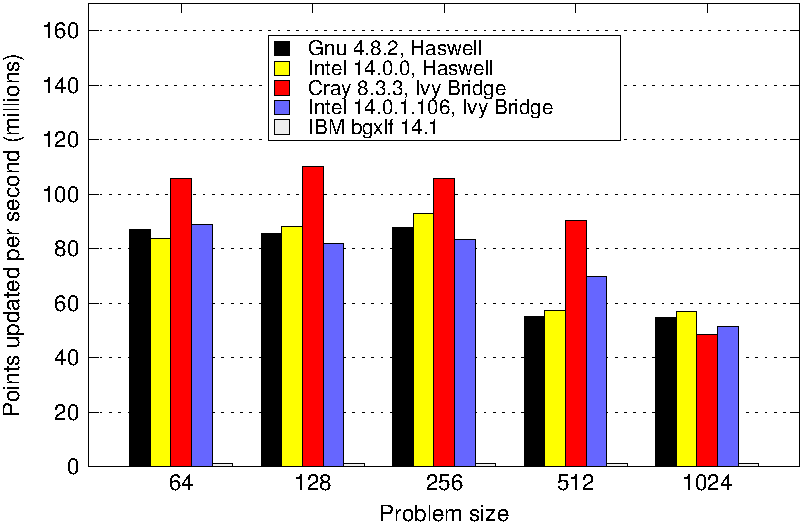
\includegraphics[width=\picwidth]{orig_summary}
\caption{Summary of the performance of the original version of the 
NEMOLite2D code on an Intel Ivy Bridge CPU for
the range of compilers under consideration.}
\label{FIG_orig_perf_summary}
\end{figure}

Moving now the to the {PS}y{KA}l version of NEMOLite2D,
Figure~\ref{FIG_best_psykal_perf_summary} plots the performance of the
fastest {PS}y{KA}l version for each of the compiler/problem-size combinations.
While the Intel compiler still produces the best-performing binary,
the Cray-compiled binary is now a very close second. In fact, the
performance of both the Gnu- and Cray-compiled {PS}y{KA}l versions is
generally significantly greater than that of their respective original
versions. We also note that best absolute performance (in terms of
grid points processed per second) with any compiler is obtained with
the $256^2$ domain.

\begin{figure}[!t]
\centering
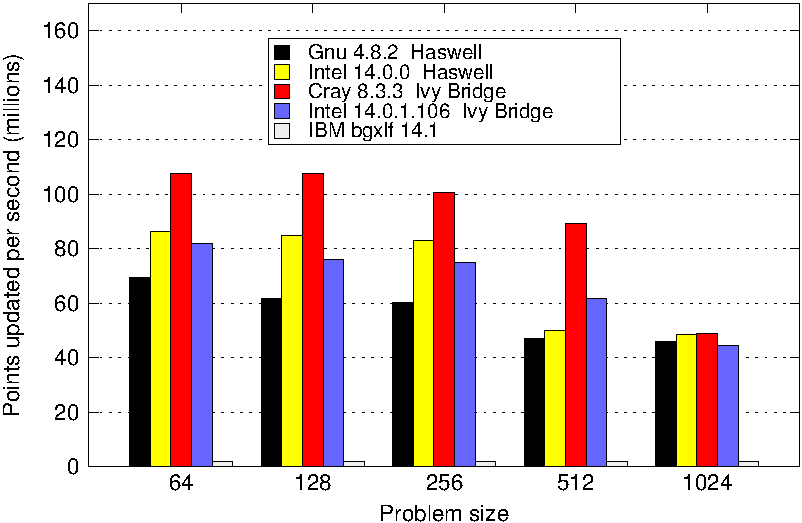
\includegraphics[width=\picwidth]{best_psykal_summary}
\caption{Summary of the best performance achieved by any {PS}y{KA}l 
version of NEMOLite2D for each of the compilers under consideration.}
\label{FIG_best_psykal_perf_summary}
\end{figure}

Figure~\ref{FIG_slowdown_summary} plots the percentage difference
between the performance of the original and the best {PS}y{KA}l versions
of NEMOLite2D for each compiler/problem-size combination. This shows that it is
only the Intel-compiled binary running the $64^2$ domain that is
slower with the {PS}y{KA}l version of the code (and then only by some
3\%). For all other points in the space, the optimised {PS}y{KA}l version
of the code performs better. The results for the Cray compiler are
however somewhat sqewed by the fact that it did not SIMD vectorise key
parts of the original version (see below).

\begin{figure}[!t]
\centering
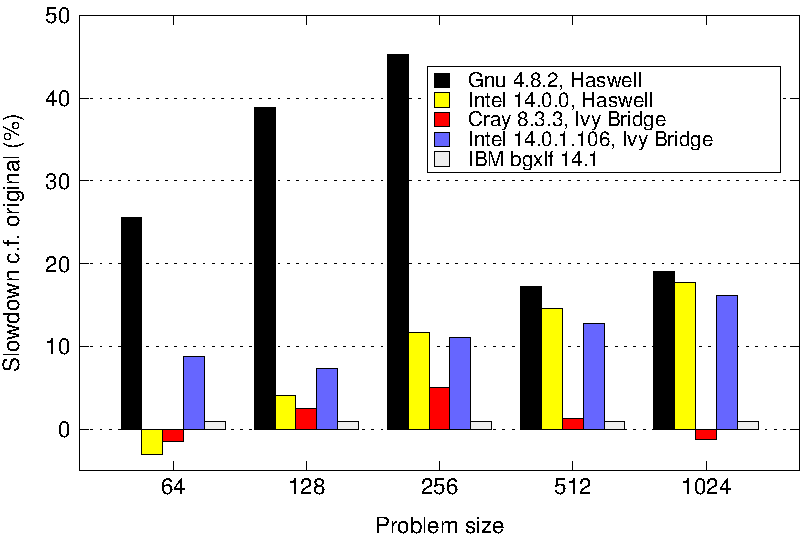
\includegraphics[width=\picwidth]{slowdown_summary}
\caption{Comparison of the performance of the best {PS}y{KA}l
version with that of the original version of the code. A negative value 
indicates that the {PS}y{KA}l version is slower than the original.}
\label{FIG_slowdown_summary}
\end{figure}

Having show that we can recover, and often improve upon, the
performance of the original version of NEMOLite2D, the next logical
step is to examine the necessary code transformations in detail.  We
do this for the $256^{2}$ case since this fits within cache on the Ivy
Bridge CPUs we are using here.  Table~\ref{TABLE_opt_breakdown} shows
detailed performance figures for this case after each transformation
has been applied to the code. The same data is visualised in
Figure~\ref{FIG_opt_stages_256}.

Looking at the results for the Gnu compiler (and the Ivy Bridge CPU)
first, all of the steps-up in performance correspond to kernel
in-lining. None of the other transformations had any effect on the
performance of the compiled code. In fact, simply in-lining the two
kernels associated with the Momentum section was sufficient to exceed
the performance of the original code.

With the Intel compiler, the single largest performance increase is
again due to kernel in-lining (of the Momentum kernels). This is
because the compiler does a much better job of SIMD vectorising the
loops involved than it does when it first has to in-line the kernel
itself (as evidenced by its own diagnostic output - see
Section~\ref{sec_inline_mom}). However, although this gives a
significant performance increase it is not sufficient to match the
performance of the original version. This is only achieved by
in-lining every kernel and making the lack of data dependencies
between arrays accessed from different field objects more explicit.

The Cray compiler is distinct from the other two in that kernel
in-lining does not give any performance benefit and in fact, for the
smaller kernels, it can actually hurt performance. Thus the key
transformation is to encourage the compiler to SIMD vectorise the
Momentum section via a compiler-specific directive (without this it
concludes that such vectorisation would be inefficient). Of the other
transformations, only the change to constant loop bounds and the
addition of the compiler-specific safe\_address directive (see
Section~\ref{sec_safe_address}) were found to (slightly) improve
performance.

\begin{table}[!t]
  \caption{Performance (millions of points updated per second) on an Intel
    Ivy Bridge CPU for the
  $256^2$ case after each code transformation. Where an optimisation
  utilises compiler-specific directives then performance figures for
  the other compilers are omitted.}
\label{TABLE_opt_breakdown}
\centering
\begin{tabular}{l|c|c|c}
\hline
Compiler:            & Gnu & Intel & Cray  \\
\hline
Original             & 3.87 & 12.2 & 6.83 \\
Vanilla {PS}y{KA}l   & 2.59 & 6.27 & 6.35 \\
Constant loop bounds & 3.07 & 6.55 & 6.73 \\
Safe-address         & --   & --   & 6.95 \\
In-line Momentum     & 4.31 & 10.7 & 6.93 \\
SIMD Momentum        & --   & --   & 11.8 \\
\parbox{2.5cm}{\raggedright Grid data from read-only objects} & 4.31 & 11.3 & 11.8 \\
In-line Continuity         & 4.83 & 11.8 & 11.6 \\
In-line remaining kernels  & 5.89 & 12.0 & 11.5 \\
In-line field copies       & 5.92 & 12.5 & 11.4 \\
\hline
\parbox{2.5cm}{\raggedright \%-speed-up of best \textit{c.f.} original} & 34.6 & 2.39 & 42.2 \\
\hline
\end{tabular}
\end{table}

\begin{figure}[!t]
\centering
\includegraphics[width=\picwidth]{opt_stages_256}
\caption{Performance of the {PS}y{KA}l version of NEMOLite2D for the
  $256^{2}$ domain at each stage of optimisation. The first (black)
  bar of each cluster gives the performance of the original version of
  NEMOLite2D for that compiler/CPU combination.}
\label{FIG_opt_stages_256}
\end{figure}

\subsection{Parallel Performance}

We now turn to transformations related to parallelisation of the
NEMOLite2D code; the introduction of OpenMP and OpenACC directives. In
keeping with the {PS}y{KA}l approach we do not modify either the
Algorithm- or Kernel-layer code.  Any code changes are restricted to
either the PSy (middle) layer or the underlying library that manages
\textit{e.g.} the construction of field objects.

\subsubsection{OpenMP}

As with the serial optimisations, we consider the effect of each of
the OpenMP optimisation steps described in Section~\ref{sec_omp_steps}
for the $256^2$ domain. For this we principally use a single Intel,
Ivy Bridge socket which has 12 hardware cores and support for up to 24
threads with hyperthreading (i.e. two threads per core).
Figures~\ref{FIG_gnu_omp_256},~\ref{FIG_intel_omp_256}
and~\ref{FIG_cray_omp_256} show the performance of each of the
versions of the code on this system for the Gnu, Intel and Cray
compilers, respectively.

In order to quantify the scaling behaviour of the different versions
of NEMOLite2D with the different compilers/run-time environments, we
also plot the parallel efficiency in
Figures~\ref{FIG_gnu_omp_256},~\ref{FIG_intel_omp_256}
and~\ref{FIG_cray_omp_256} (dashed lines and open symbols). We define
parallel efficiency (\%), $E(n)$, on $n$ threads, as:
\[
E(n) = 100  \frac{P(n)}{ n P(1)}
\]
where $P(n)$ is the performance of the code on $n$ threads,
\textit{e.g.} grid-points updated per second. For a
perfect, linearly-scaling code, $E(n)$ will be 100\%.

Since the space to explore consists of three different compilers, six
different domain sizes, five stages of optimisation and six different
thread counts we can only consider a slice through it in what follows.
In order to inform our choice of domain size,
Figure~\ref{FIG_omp_domain_size} shows the scaling behaviour of the
most performant, Intel-compiled version of NEMOLite2D. Although it is
common for production runs of NEMO to use MPI sub-domains of $20
\times 20$, it is clear from Figure~\ref{FIG_omp_domain_size} that the
limited quantity of parallelism in the $32 \times 32$ domain inhibits
scaling. Therefore, to fully test the performance of our OpenMP
implementations we have chosen to examine results for the $256 \times
256$ domain and these are shown in Figures~\ref{FIG_gnu_omp_256},
\ref{FIG_intel_omp_256} and \ref{FIG_cray_omp_256}.

\begin{figure}
\centering
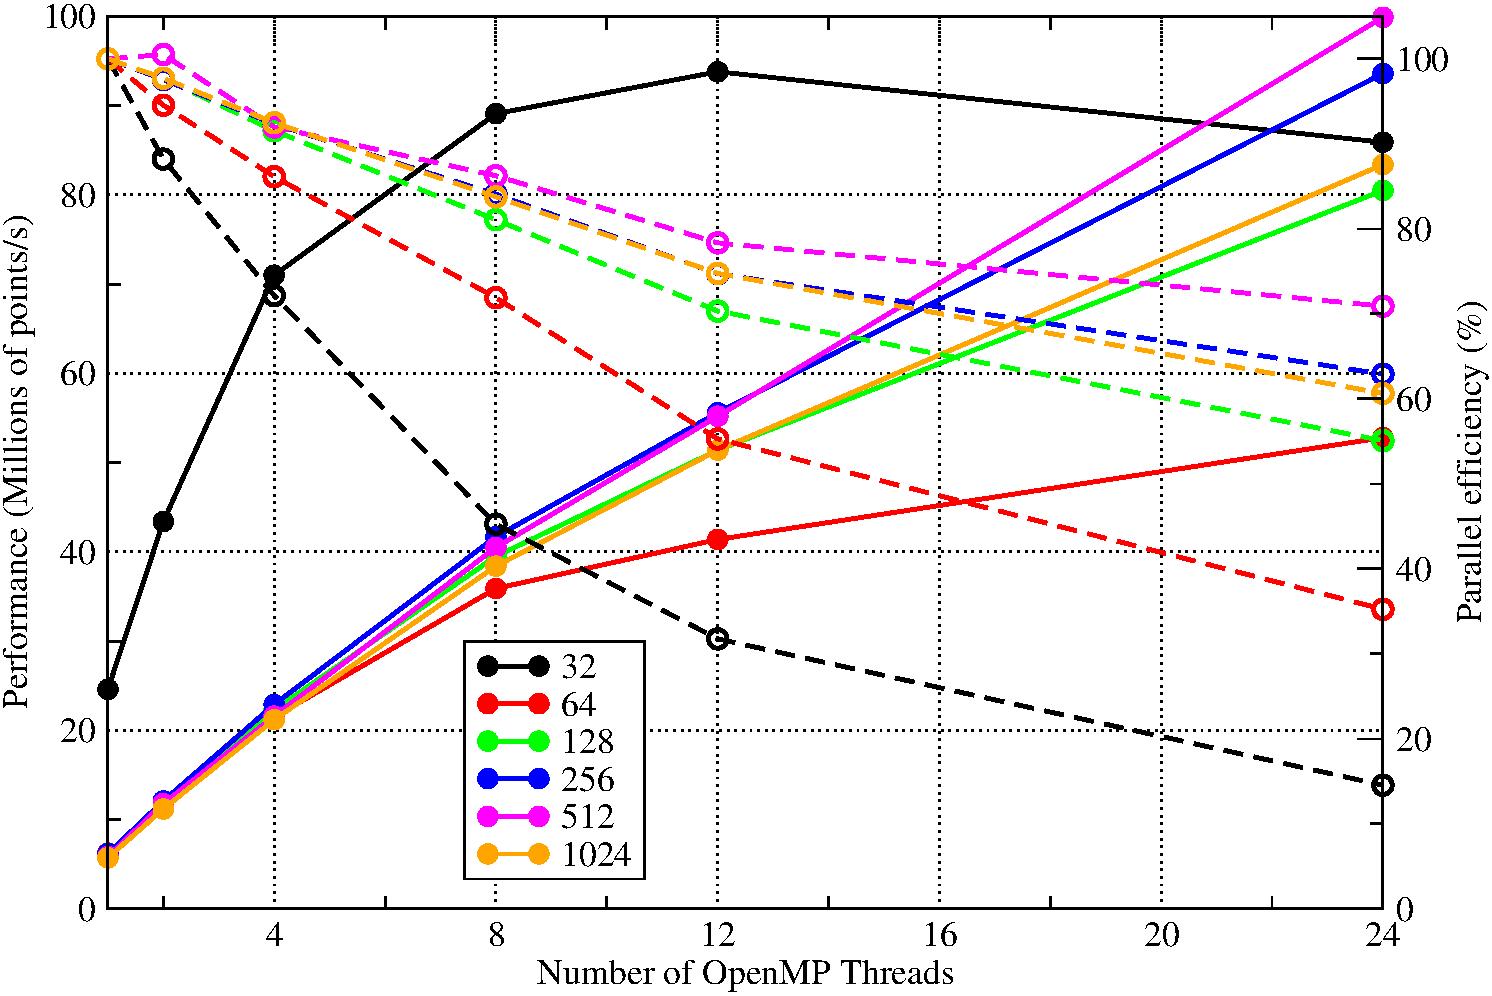
\includegraphics[width=\picwidth]{omp_scaling_problem_size}
\caption{The scaling behaviour of the most performant OpenMP-parallel
  version of {PS}y{KA}l NEMOLite2D for the full range of domain sizes
  considered on the CPU. Results are for the Intel compiler on a
  single Intel Ivy Bridge socket. The corresponding parallel
  efficiencies are shown using open symbols and dashed lines. The
  24-thread runs employed hyperthreading.}
\label{FIG_omp_domain_size}
\end{figure}

\begin{figure}
\centering
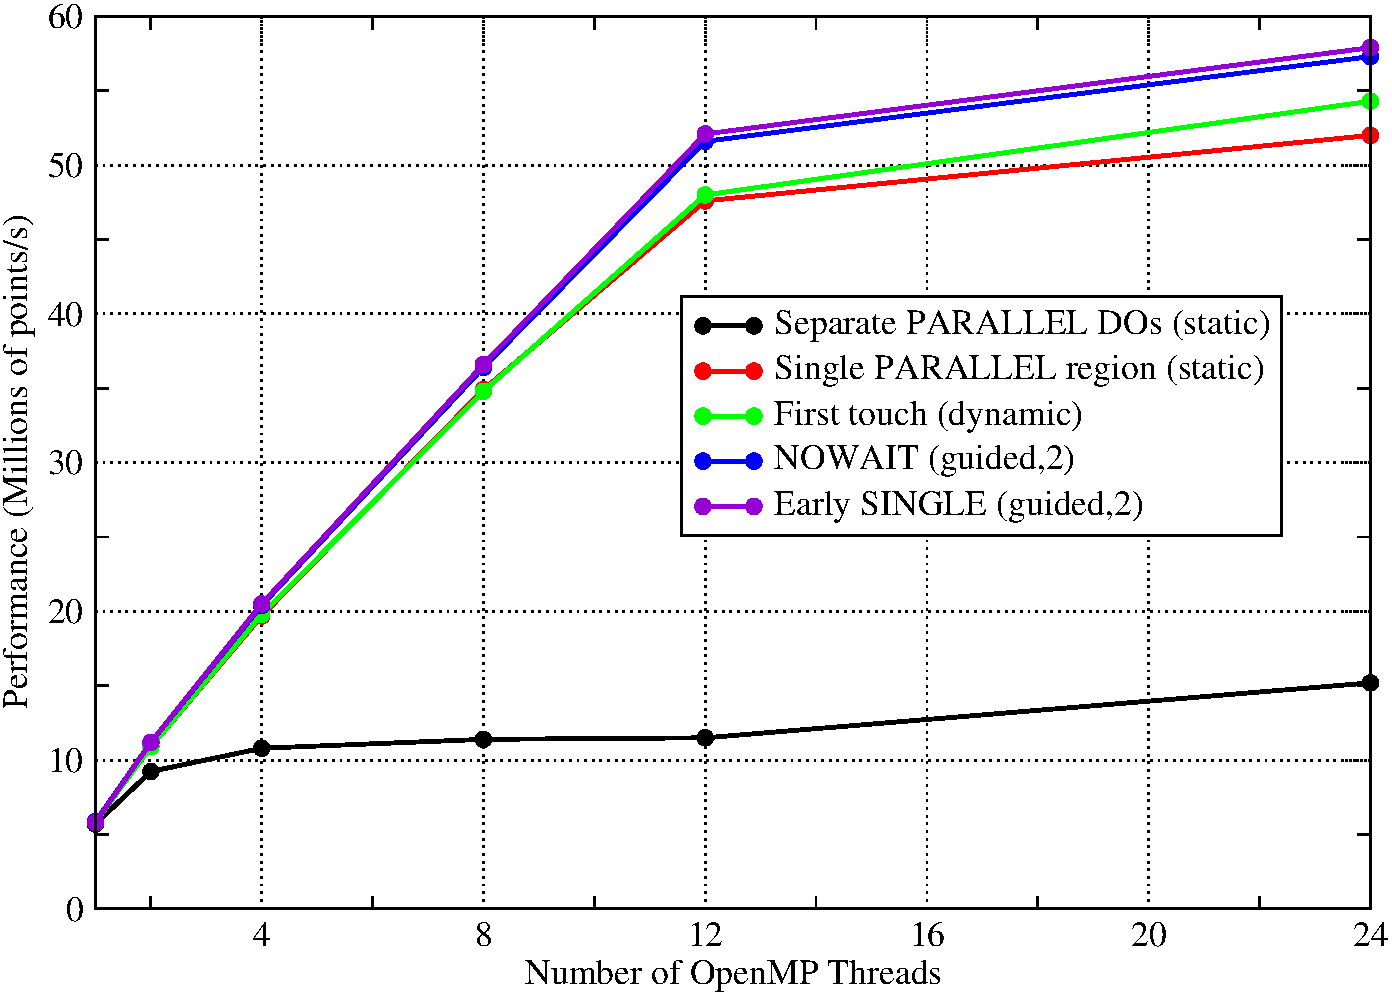
\includegraphics[width=\picwidth]{omp_scaling_256_gnu}
\caption{Performance of the OpenMP-parallel version of
  {PS}y{KA}l NEMOLite2D for the $256^2$ domain with the Gnu compiler on
  a single Intel Ivy Bridge socket. The corresponding parallel
  efficiencies are shown using open symbols and dashed lines. The
  24-thread runs employed hyperthreading and the optimal OpenMP
  schedule is given in parentheses.}
\label{FIG_gnu_omp_256}
\end{figure}

The simplest OpenMP implementation (black lines, circle symbols) fails
to scale well for any of the compilers. For the Intel and Gnu
versions, parallel efficiency is already less than 50\% on just four
threads. The Cray version however does better and is about 45\%
efficient on eight threads (right axis, Figure~\ref{FIG_cray_omp_256}).

With the move to a single PARALLEL region, the situation
is greatly improved with all three executables now scaling out to at
least 12 threads with $\sim70$\% efficiency (red lines, square symbols).

In restricting ourselves to a single socket, we are keeping all
threads within a single NUMA region. It is therefore surprising that
implementing a `first-touch' policy has any effect and yet, for the
Gnu- and Intel-compiled binaries, it appears to improve performance
when hyperthreading is employed to run on 24 threads (green lines and
diamond symbols in Figures~\ref{FIG_gnu_omp_256} and
~\ref{FIG_intel_omp_256}).

\begin{figure}
\centering
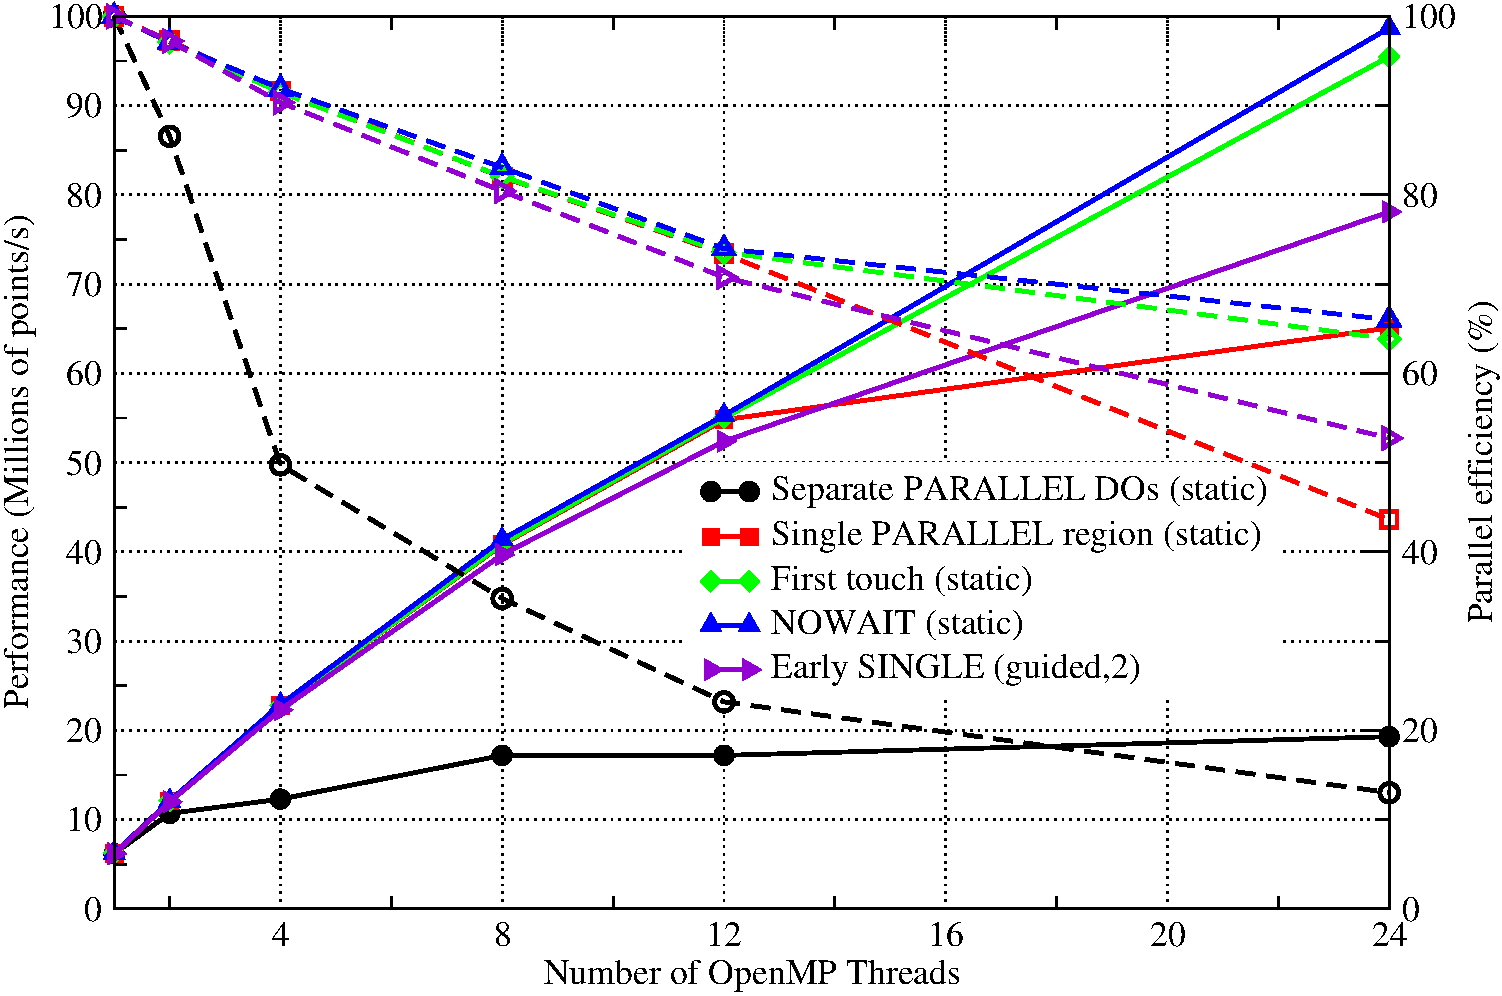
\includegraphics[width=\picwidth]{omp_scaling_256_intel}
\caption{Performance of the OpenMP-parallel version of {PS}y{KA}l
  NEMOLite2D for the Intel compiler on a single Intel Ivy Bridge
  socket.  The corresponding parallel efficiencies are shown using
  open symbols and dashed lines. The 24-thread runs employed
  hyperthreading and the optimal OpenMP schedule is given in
  parentheses.}
\label{FIG_intel_omp_256}
\end{figure}

\begin{figure}
\centering
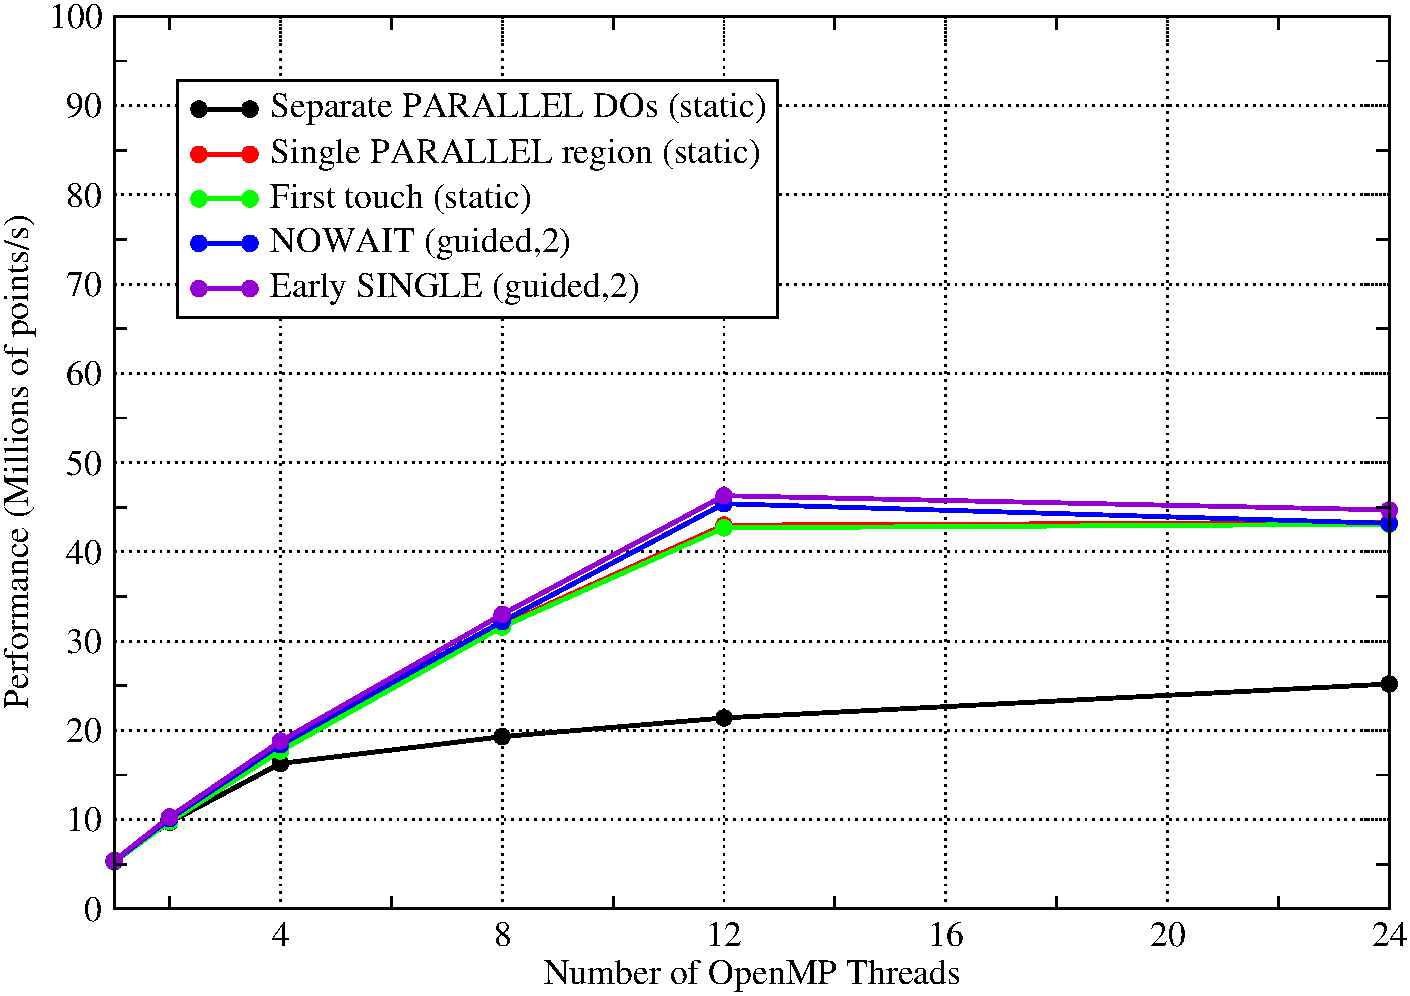
\includegraphics[width=\picwidth]{omp_scaling_256_cray}
\caption{Performance of the OpenMP-parallel version of {PS}y{KA}l
  NEMOLite2D for the Cray compiler on a single Intel Ivy Bridge
  socket.  The corresponding parallel efficiencies are shown using
  open symbols and dashed lines. The 24-thread runs employed
  hyperthreading and the optimal OpenMP schedule is given in
  parentheses.}
\label{FIG_cray_omp_256}
\end{figure}

The final optimisation step that we found to have any significant
effect is to minimise the amount of thread synchronisation by
introducing the NOWAIT qualifier wherever possible (blue lines and
upwards-triangle symbols). For the Gnu compiler, this improves the
performance of the executable on eight or more threads while, for the
Intel compiler, it only gives an improvement for the 24-thread
case. Moving the SINGLE region before a parallel loop is marginally
beneficial for the Gnu- and Cray-compiled binaries and yet reduces the
performance of the Intel binary (purple lines and right-pointing
triangles).

We have used different scales for the $y$-axes in each of the plots in
Figures~\ref{FIG_gnu_omp_256},~\ref{FIG_intel_omp_256}
and~\ref{FIG_cray_omp_256} in order to highlight the performance
differences between the code versions with a given compiler. However,
the best performance obtained on twelve threads (\textit{i.e.}  without
hyperthreading) is 52.1, 55.6 and 46.3 (million points/s) for the Gnu,
Intel and Cray compilers, respectively. This serves to emphasise the
democratisation that the introduction of OpenMP has had; for the
serial case the Cray- and Intel-compiled exectables were a factor of
two faster than the Gnu-compiled binary
(Figure~\ref{FIG_opt_stages_256}). In the OpenMP version, the
Gnu-compiled binary is only 6\% slower than that produced by the Intel
compiler and is 13\% \textit{faster} that that of the Cray compiler. In
part this situation comes about because of the effect that adding the
OpenMP compiler flag has on the optimisations performed by the
compiler.  In particular, the Cray compiler no longer vectorises the
key Momentum section, despite the directive added during the serial
optimisation work. This defficiency has been reported to Cray.

Since NEMO and similar finite-difference codes tend to be
memory-bandwidth bound, we checked the sensitivity of our performance
results to this quantity by benchmarking using two sockets of Intel
Ivy Bridge (\textit{i.e.} using a complete node of ARCHER, a Cray
XC30). For this configuration we ensured that threads were evenly
shared over the two sockets. The performance obtained for the $256^2$
case with the `early SINGLE' version of the code is compared with the
single-socket performance in
Figure~\ref{FIG_omp_2socks}. Surprisingly, doubling the available
memory bandwidth in this way has little effect on performance - the
two-socket performance figures track those from a single socket very
closely. The only significant difference in performance is at 24
threads where, in addition to the difference in available memory
bandwidth, the single-socket configuration is using hyperthreading
while the two-socket case is not.  The discrepancy in the performance
of the Cray- and Intel-compiled binaries at this thread count is under
investigation by Cray.

\begin{figure}
\centering
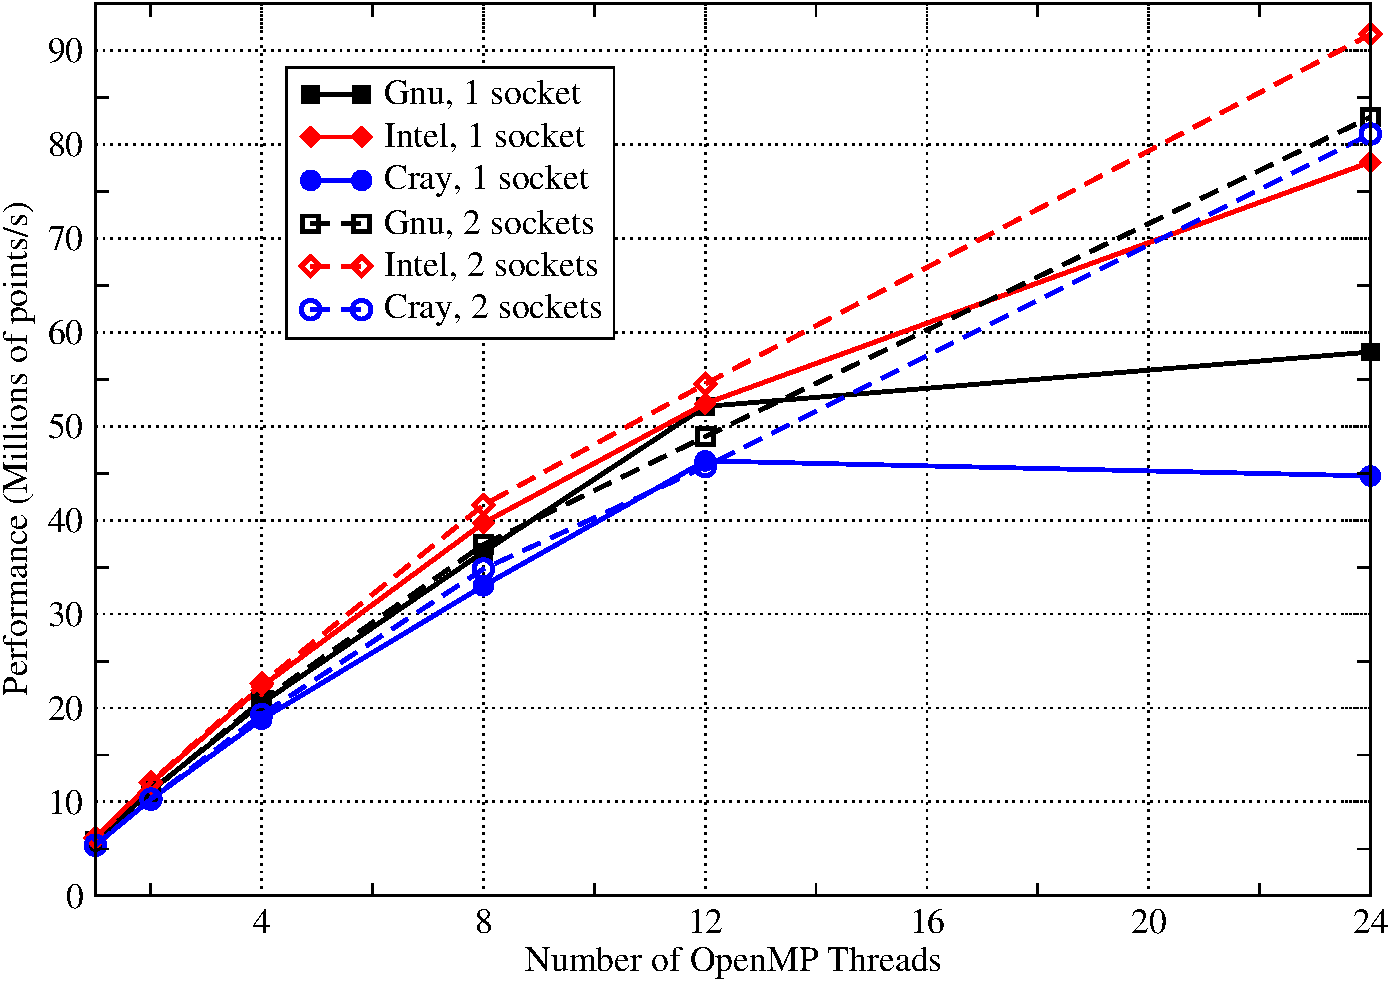
\includegraphics[width=\picwidth]{1and2sockets}
\caption{Performance of the OpenMP-parallel version of {PS}y{KA}l
  NEMOLite2D on one and two sockets of Intel Ivy Bridge. The 24-thread
  runs on a single socket used hyperthreading and the two-socket runs
  had the threads shared equally between the sockets.}
\label{FIG_omp_2socks}
\end{figure}

A further complication is the choice of scheduling of the OpenMP
threads.  We have investigated the performance of each of the
executables (and thus the associated OpenMP run-time library) with the
standard OpenMP \textit{static}, \textit{dynamic} and \textit{guided}
scheduling policies. For the Intel compiler/run-time, static loop
scheduling was found to be best for all versions apart from that where
we have attempted to amortize the cost of the SINGLE section. This is
to be expected since that strategy requires some form of dynamic loop
scheduling in order to reduce the load imbalance introduced by the
SINGLE section.

In contrast, some form of dynamic scheduling gave a performance
improvement with the Gnu compiler/run-time even for the `first-touch'
version of the code. This is despite the fact that this version
contains (implicit) thread synchronisation after every parallel loop.
For the Cray compiler/run-time, some form of dynamic scheduling became
optimal once inter-thread synchronisation was reduced using the NOWAIT
qualifiers.


%\begin{figure}
%\centering
%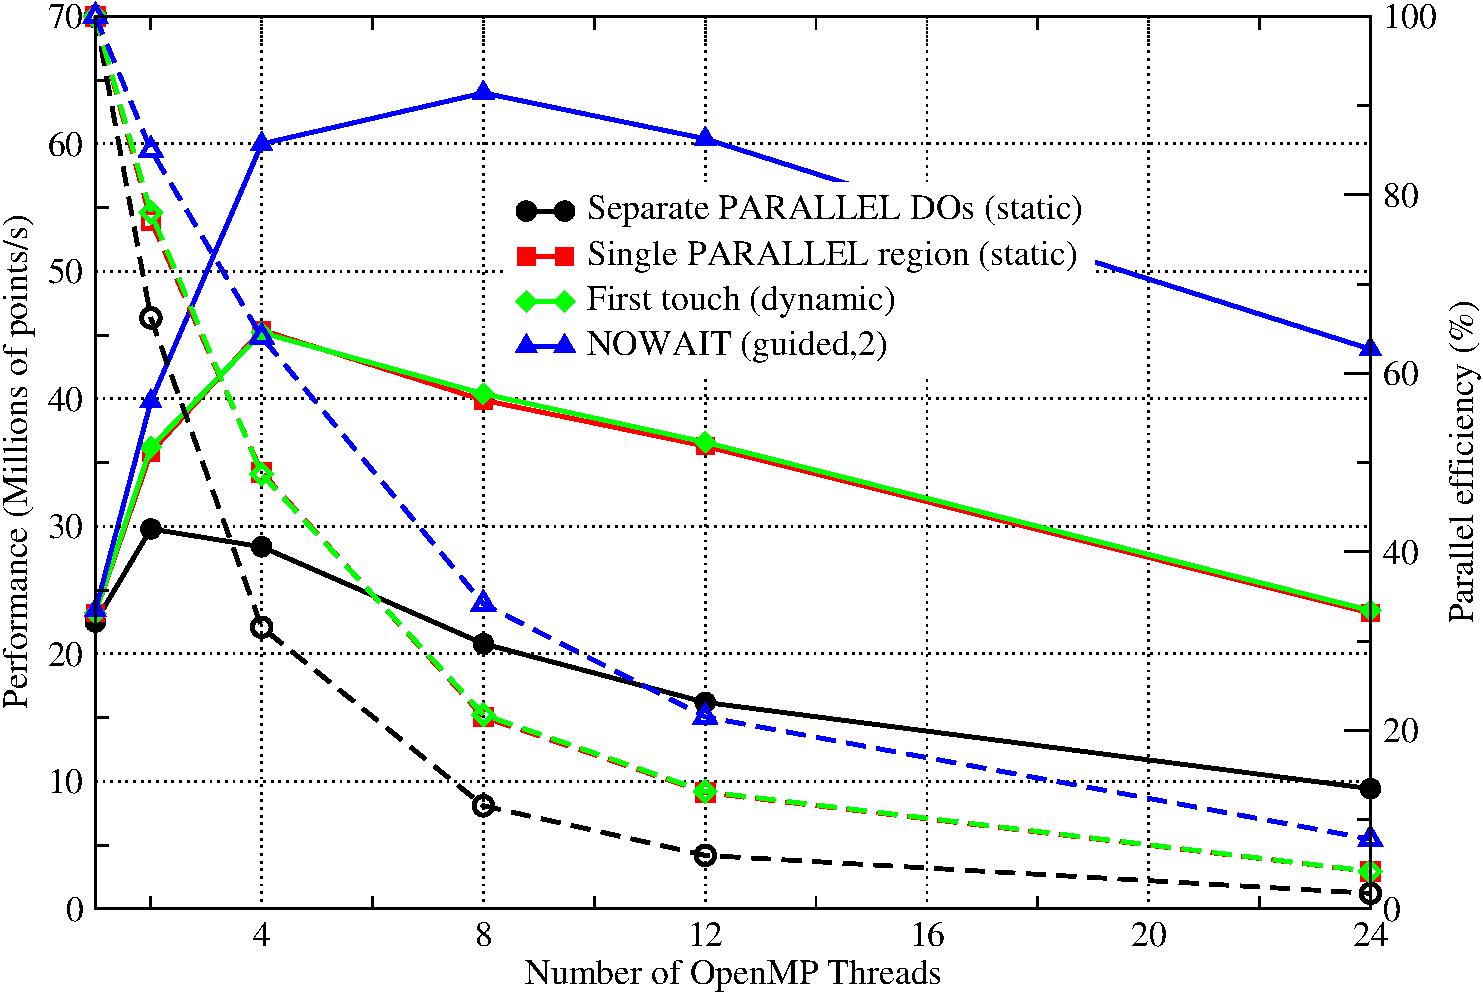
\includegraphics[width=\picwidth]{omp_scaling_32_gnu}
%\caption{Performance of the OpenMP-parallel version of {PS}y{KA}l
%  nemolite2d for the Gnu compiler on a single Intel Ivy Bridge
%  socket. The corresponding parallel efficiencies are shown using open
%  symbols and dashed lines. The 24-thread runs employed hyperthreading
%  and the optimal OpenMP schedule is given in parentheses.}
%\label{FIG_gnu_omp_32}
%\end{figure}

%\begin{figure}
%\centering
%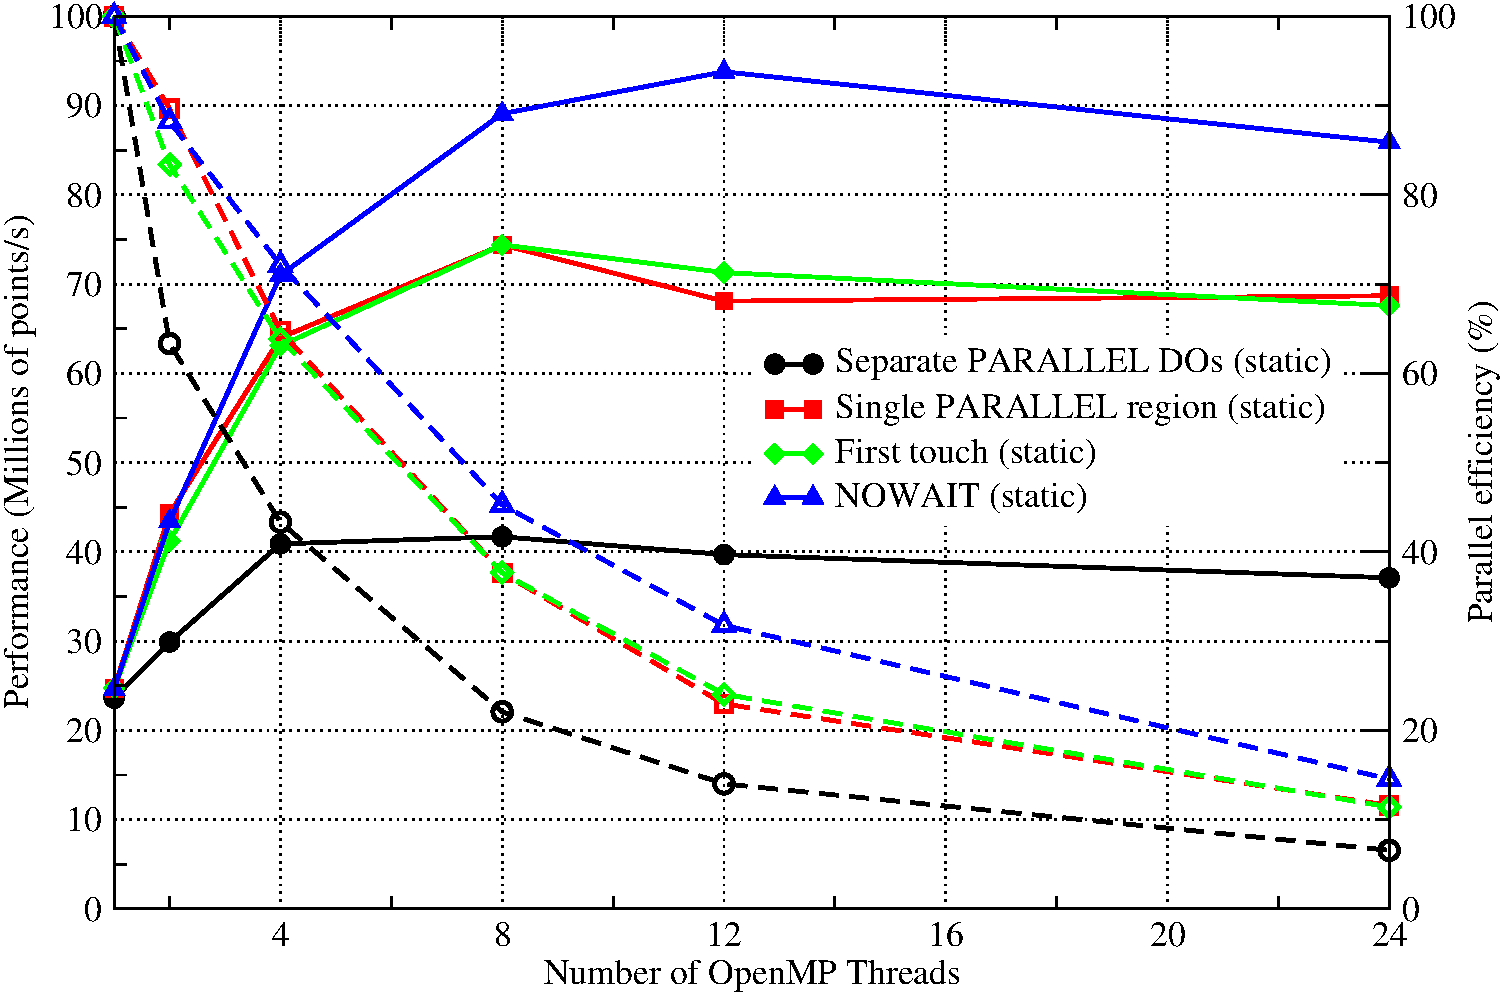
\includegraphics[width=\picwidth]{omp_scaling_32_intel}
%\caption{Performance of the OpenMP-parallel version of {PS}y{KA}l
%  nemolite2d for the Intel compiler on a single Intel Ivy Bridge
%  socket.  The corresponding parallel efficiencies are shown using
%  open symbols and dashed lines. The 24-thread runs employed
%  hyperthreading and the optimal OpenMP schedule is given in
%  parentheses.}
%\label{FIG_intel_omp_32}
%\end{figure}

%\begin{figure}
%\centering
%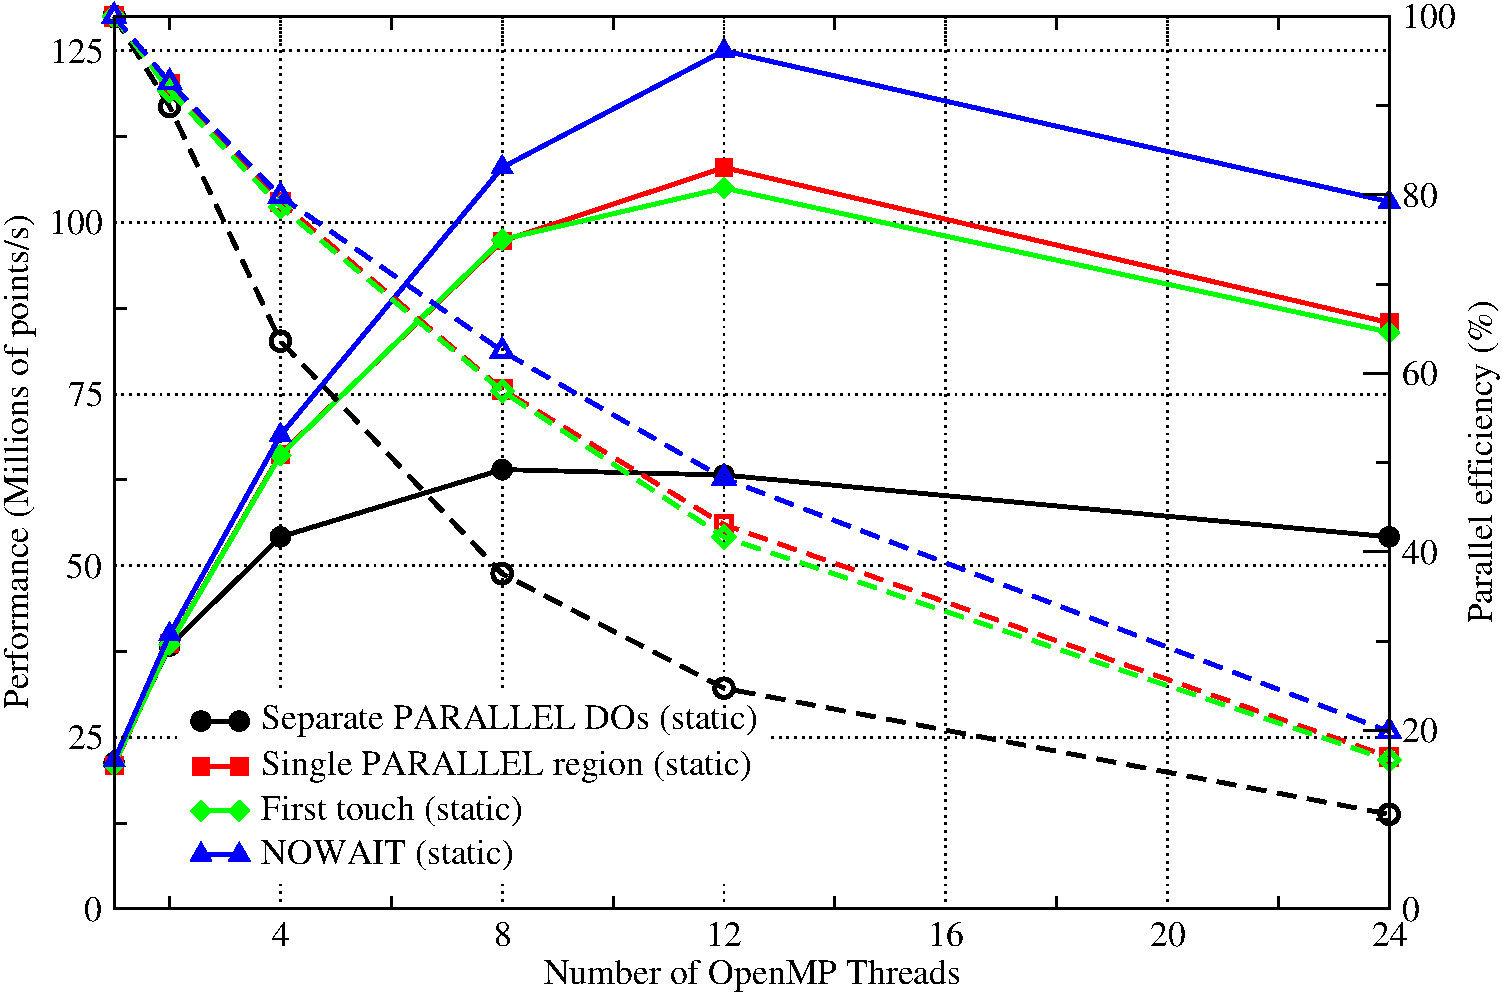
\includegraphics[width=\picwidth]{omp_scaling_32_cray}
%\caption{Performance of the OpenMP-parallel version of {PS}y{KA}l
%  nemolite2d for the Cray compiler on a single Intel Ivy Bridge
%  socket.  The corresponding parallel efficiencies are shown using
%  open symbols and dashed lines. The 24-thread runs employed
%  hyperthreading and the optimal OpenMP schedule is given in
%  parentheses.}
%\label{FIG_cray_omp_32}
%\end{figure}

\subsubsection{OpenACC}

The advantage of the {PS}y{KA}l re-structuring becomes apparent if we
wish to run NEMOLite2D on different hardware, \textit{e.g.} a
GPU. This is because the necessary code modifications are, by design,
limited to the middle PSy layer. In order to demonstrate this and to
check for any limitations imposed by the {PS}y{KA}l re-structuring, we
had a GPU expert from NVIDIA port the Fortran NEMOLite2D to GPU. He
used OpenACC directives for this porting as that approach is similar
to the use of OpenMP directives and works well within the {PS}y{KA}l
apprach. He also experimented with using CUDA directly within the
original form of NEMOLite2D in order to quantify any performance
penalty incurred by taking the {PS}y{KA}l/OpenACC approach.

The performance of these two versions of the code is plotted in
Figure~\ref{FIG_gpu_opt_stages}.  Since the {PS}y{KA}l restructuring of
NEMOLite2D did not prove to be a barrier to achieving a performant
code when using OpenACC directives, we only report the performance of
the {PS}y{KA}l OpenACC version. For problem sizes up to $256^2$ the
difference in the performance of the two versions is less than 5\% and
for the larger domains it is at most 11\%. This demonstrates that the
performance cost of the {PS}y{KA}l approach in utilising a GPU for
NEMOLite2D is minimal.

\begin{figure}
\centering
\includegraphics[width=\picwidth]{gpu_opt_stages}
\caption{Performance of the {PS}y{KA}l (OpenACC) and CUDA GPU
  implementations of NEMOLite2D. The performance for the OpenACC
  version of the original code is not shown since it is identical to
  that of the {PS}y{KA}l version.}
\label{FIG_gpu_opt_stages}
\end{figure}

In Figure~\ref{FIG_cpu_cf_gpu} we compare the absolute performance of
the OpenMP and OpenACC implementations of NEMOLite2D across the range
of problem sizes considered. The OpenMP figures are the maximum
performance obtained from a whole Intel Ivy Bridge socket by any
version of the code on any number of threads for a given
compiler/run-time. For the smallest domain size ($64^2$) the OpenMP
version significantly outperforms the GPU because there is
insufficient parallelism to fully utilise the GPU and one time-step
takes only 80~$\mu$s. The execution of a single time-step is then
dominated by the time taken to launch the kernels on the GPU rather than
the execution of the kernels themselves.

\begin{figure}
\centering
\includegraphics[width=\picwidth]{cpu_cf_gpu}
\caption{Performance of the best OpenMP-parallel version of {PS}y{KA}l\
  NEMOLite2D (on a single Intel Ivy Bridge socket) compared with the {PS}y{KA}l GPU implementation (using OpenACC).}
\label{FIG_cpu_cf_gpu}
\end{figure}

Once the problem size is increased to $128^2$, a single time-step
takes roughly 200~$\mu$s and only the Intel-compiled OpenMP version is
comparable in performance to the OpenACC version. For all of the
larger problem sizes plotted in Figure~\ref{FIG_cpu_cf_gpu} the GPU
version is considerably faster than the CPU.  For problem sizes of
$1024^2$ and greater, the 30MB cache of the Ivy Bridge CPU is
exhausted and performance becomes limited by the bandwidth to main
memory. At this stage the OpenACC version of the code on the GPU is
some 3.4 times faster than the best OpenMP version on the CPU.

%Peak memory bandwidth on the K40 GPU is 288 GB/s and we measured
%(using STREAM2) bandwidths of 46.0 and 20.5 GB/s to L3 and main
%memory, respectively on the CPU.

\subsection{Performance Analysis with the Roofline Model}

Although we have investigated how the performance of the {PS}y{KA}l
version of NEMOLite2D compares with that of the original, we have not
addressed how efficient the original actually is. In order to do so we
use the Roofline Model~\citep{roofline} which provides a relatively
simple way of characterising the performance of a code in terms of
whether it is memory-bandwidth bound or compute bound. To do so we
follow the approach suggested in~\cite{para_pearls} and use the
STREAM~\citep{stream} and LINPACK~\citep{linpack} benchmarks in order to
get the upper bounds on the memory bandwidth and floating-point
operations per second (FLOPS) for the test hardware. Since we are
using an Intel Ivybridge CPU we used the Intel Math Kernel Library
implementation of LINPACK.

A key component of the Roofline model is the Operational or Arithmetic
Intensity of the code being executed:
\[
AI = \frac{\textrm{No. of floating-point operations}}{\textrm{Bytes fetched from memory}}
\]
We calculated this quantity manually by examining the
source code and counting the number of memory references and
arithmetic operations that it contained. In doing this counting we
assume that any references to adjacent array elements (\textit{e.g.}
$u(i,j)$ and $u(i+1,j)$) are fetched in a single cache line and thus
only count once.

\begin{figure}
\centering
\includegraphics[width=\picwidth]{roofline}
\caption{Comparison of the performance achieved by kernels from
  NEMOLite2D and Shallow on a roof-line plot for the E5-1620
  CPU. Results for the former are for the $256^2$ domain since that
  gave the best performance. See the text for a discussion of the
  different CPU ceilings (dashed lines).}
\label{FIG_roofline}
\end{figure}

In Figure~\ref{FIG_roofline} we show the performance of kernels from
both Shallow and NEMOLite2D on the roofline model for an Intel E5-1620 CPU.
This demonstrates that the Shallow kernel is achieving a performance
roughly consistent with saturating the available memory bandwidth. In
contrast, the kernel taken from NEMOLite2D is struggling to reach a
performance consistent with saturating the bandwidth to main
memory. We experimented with reducing the problem size (so as to
ensure it fitted within cache) but that did not significantly improve
the performance of the kernel. This then points to more fundamental issues
with the way that the kernel is implemented which are not captured in the
simple roofline model.

In order to aid our understanding of kernel performance we have
developed a tool capable of parsing Fortran code and generating a
Directed Acyclic Graph (DAG) of the data flow. This tool eases the
laborious and error-prone process of counting memory accesses and
FLOPs as well as providing information on those operations that are
rate-limiting or on the critical path. Using the details of the Intel
Ivy Bridge microarchitecture published by Fog~\citep{fog_microarch,
  fog_instructions} we have constructed performance estimates of the
NEMOLite2D kernel. By ignoring all Instruction-Level Parallelism
(ILP), \textit{i.e.} assuming that all nodes in the DAG are executed
in serial, we get a lower-bound performance estimate of $0.6391 \times
CLOCK\_SPEED$ FLOPS which gives 2.46~GFLOPS at a clock speed of
3.85~GHz.

Alternatively, we may construct an upper bound by assuming the
out-of-order execution engine of the Ivy Bridge core is able to
perfectly schedule and pipeline all operations such that those that go
to different execution ports are always run in parallel. In the Ivy
Bridge core, floating-point multiplication and division operations go
to port 0 while addition and subtraction go to port
1~\citep{fog_instructions}. Therefore we sum the cost of all
multiplication and division operations in the DAG and compare that
with the sum of all addition and subtraction operations. The greater
of these two quantities is then taken to be the cost of executing the
kernel; all of the operations on the other port are assumed to be done
in parallel. This gives a performance estimate of $1.029 \times
CLOCK\_SPEED$ FLOPS or 3.96 GFLOPS at 3.85~GHz.

These performance estimates are plotted as CPU ceilings (horizontal
dashed lines) in Figure~\ref{FIG_roofline}. The performance of the
Momentum kernel is seen to fall between these two bounds which
demonstrates that its performance is not memory-bandwidth limited, as
might have been assumed by its low AI. Therefore, although the
performance of this kernel is clearly sub-optimal, this is due to the
balance of floating-point operations that it contains. Improving this
is outside the scope of the current work since here we are focused on
the {PS}y{KA}l separation of concerns and the introduction of parallelism
in the PSy layer.

Enabling SIMD vectorisation for this kernel does not significantly
improve its performance (Figure~\ref{FIG_roofline}) and in fact,
limiting it to SSE instructions (vector width of two double-precision
floating point numbers) rather than AVX (vector width of four) was
found to produce a slightly more performant version. The poor
efficiency of the SIMD version is highlighted by the fact that the
corresponding kernel performance no longer falls within the bounds of
our performance estimate. This is because we have incorporated the
effect of SSE into that estimate by simply assuming perfect
vectorisation which gives a performance increase of a factor of two.

%%%%%%%%%%%%%%%%%%%%%%%%%%%%%%%%%%%%%%%%%%%%%%%%%%%%%%%%%%%%%%%%%%%%
\conclusions

We have investigated the application of the {PS}y{KA}l separation of
concerns approach to the domain of shared-memory parallel,
finite-difference shallow-water models. This approach enables the
computational science (performance) related aspects of a computer
model to be kept separate from the natural (oceanographic) science
aspects.

We have used a new and un-optimised, two-dimensional model extracted
from the NEMO ocean model for this work. As a consequence of this, the
introduction of the {PS}y{KA}l separation of concerns followed by
suitable transformations of the PSy Layer is actually found to improve
performance. This is in contrast to our previous
experience~\citep{shallow_psykal} with tackling the Shallow code which
has been optimised over many years. In that case we were able to
recover (to within a few percent) the performance of the original and
in some cases exceed it, in spite of limiting ourselves to
transformations which replicated the structure of the original,
optimised code.

Investigation of the absolute serial performance of the NEMOLite2D
code using the roofline model revealed that it was still significantly
below any of the traditional roofline ceilings. We have developed
Habakkuk (https://github.com/arporter/habakkuk), a code-analysis tool
that is capable of providing more realistic ceilings by analysing the
nature of the floating point computations performed by a kernel. The
bounds produced by Habakkuk are in good agreement with the measured
performance of the principal (Momentum) kernel in NEMOLite2D. In
future work we aim to extend this tool to account for SIMD operations
and make it applicable to code parallelised using OpenMP.

The application of code transformations to the middle/PSy layer is key
to the performance of the {PS}y{KA}l version of a code. For both
NEMOLite2D and Shallow we have found that for serial performance, the
most important transformation is that of in-lining the kernel source
at the call site, i.e. within the PSy layer. (Although we have done
this in-lining manually for this work, our aim is that in future, such
transformations will be performed automatically at compile-time and
therefore do not affect the code that a scientist writes.)
For the more complex NEMOLite2D code the Cray compiler also
had to be coerced into performing SIMD vectorisation through the use
of souce-code directives.

In this work we have also demonstrated the introduction of parallelism
into the PSy layer with both OpenMP and OpenACC directives. In both
cases we were able to leave the natural-science parts of the code
unchanged. For OpenMP we achieved a parallel efficiency of $\sim70\%$
on 12 threads by enclosing the body of the (single) PSy layer routine
within a single PARALLEL region. Removal of unecessary synchronisation
points through use of the NOWAIT clause boosted 12-thread performance
by approximately 10\% with the Gnu and Cray compilers. The
{PS}y{KA}l re-structuring of this (admittedly small) code was not found
to pose any problems for the introduction of performant OpenMP.
Similarly, we have also demonstrated good GPU performance using OpenACC
in a {PS}y{KA}l version of the code.

This paper demonstrates that the {PS}y{KA}l separation of concerns may
be applied to 2D finite-difference codes without loss of
performance. We have also shown that the resulting code is amenable to
efficient parallelisation on both GPU and shared-memory CPU systems.
This then means that it is possible to achieve performance portability
while maintaining single-source science code.

Our next steps will be first, to consider the automatic generation of the
PSy layer and second, to look at extending the approach to the full NEMO
model (i.e. three dimensions). In future work we will analyse the
performance of a domain-specific compiler that performs the automatic
generation of the PSy layer. This compiler (which we have named
`PSyclone', see https://github.com/stfc/psyclone) is currently under
development.

\codeavailability{The NEMOLite2D package is available as the GOcean
 2.0 benchmark, available from https://puma.nerc.ac.uk/trac/GOcean.}

\competinginterests{No competing interests are present.}

%%%%%%%%%%%%%%%%%%%%%%%%%%%%%%%%%%%%%%%%%%%%%%%%%%%%%%%%%%%%%%%%%%%%
\begin{acknowledgements}

This work made use of the ARCHER UK National Supercomputing Service
(\url{http://www.archer.ac.uk}) and Emerald, a GPU-accelerated High
Performance Computer, made available by the Science \& Engineering
South Consortium operated in partnership with the STFC
Rutherford-Appleton Laboratory
(\url{http://www.ses.ac.uk/high-performance-computing/emerald/}).

\end{acknowledgements}

\bibliographystyle{copernicus}
\bibliography{nemolite2d_perf}

\end{document}


